% !Mode:: "TeX:UTF-8"

\chapter[马尔科夫链蒙特卡洛算法并行化]{马尔科夫链蒙特卡洛算法并行化}
    贝叶斯网络是人工智能领域中用来处理不确定性问题的一个重要工具,其在解决问题时,概率推理是需要解决的首要问题。
叶斯网络推理关心在给定的一组证据变量值的情况下,特定变量的后验概率分布。贝叶斯网络的任何精确推理都是NP难问题,所以考虑近似
推理方法是一个高效的选择。马尔科夫链蒙特卡洛算法作为应用广泛的贝叶斯网络推力技术之一,可以在确定用户目前样本的
基础下,提供后验分布直接抽样的途径,得到未来的量,从而隐含地求解积分。

马尔科夫链蒙特卡罗算法有两部分构成:一: 马尔科夫链 ;二 :蒙特卡洛积分。
\section{蒙特卡洛算法介绍}
    蒙特卡罗方法(Monte Carlo method)又称为统计模拟方法。蒙特卡洛算法始发于20世纪40年代的美国原子弹制造曼哈顿计划,
有众多数学家和计算科学家参与, 当时由于计算机技术的发展和电子计算机的发明,使得概率统计理论为指导的数值计算方法能够
得到有效解决。蒙特卡洛算法在研究裂变物质的中子连锁反应的时开始应用,并在最早的计算机上进行编程实现。蒙特卡罗算法的本质
是使用随机数(或者伪随机数)来解决计算问题,是以概率为基础的方法。属于随机行算法,与之对应的为确定性算法。蒙特卡罗算法在金
融工程学,宏观经济学,生物医学,计算物理学等等领域都有广泛的应用。

    统计模拟中一个重要的问题是在计算机中生成一个概率分布p(x)的样本。均匀分布Uniform(0,1)的样本是相对容易生成的。 
线性同余发生器可以用来生成伪随机数,采用确定性算法生成[0,1]之间的伪随机数序列,生成序列的各种统计指标和均匀分布
结果非常接近。这些随机数可以当成真实的随机数.如图 ~\ref{fig:px}所示,

    \begin{figure}[htbp]
    \centering
    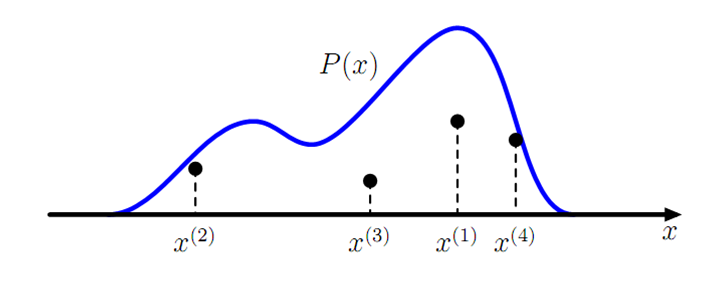
\includegraphics[width=0.8\textwidth]{px}
    \caption{伪随机数生成的概率分布的样本}\label{fig:px}
    \vspace{\baselineskip}
    \end{figure}

    但当p(x)的形式很复杂,或者p(x)是个高维的分布的时候,生成样本会很困难。在使用蒙特卡洛积分算法时,以抽样平均的方式计算
    下值$$E[\Theta|y] \simeq \frac{1}{n} \sum_{t=1}{n}\Theta_t|y$$,其中样本$\{\Theta_t|t=1,2,\ldots,n\}$来自概率密度函数
为$P(\Theta|y)$原本,即采用样本的平均数来估计期望值。当样本的总数$n$够大时,样本的平均数接近于原样本的均数。
    
    蒙特卡洛算法让积分变得简单,但实际上当$p(\Theta|y)$不是一般标准的分配时,需要更复杂的算法来产生样本。马尔科夫链的作用
开始体现。

\section{马尔科夫链介绍}
   一般情况下,随机过程在某个时刻的状态仅仅与前一个状态有关,时间相隔越远,状态之间的关联度越小,经过数学抽象,可以得到马尔科夫链。

    马尔科夫链的核心思想是:在给定的当前知识或者信息的情况下,只有用当前的状态用来预测未来,过去(即当前
以前的历史状态)对于预测将来(即当前以后的未来状态)是无关的.可以理解为某个随机过程,给了
当前时间节点的$X_i$,若$X_s(s>t)$的值不受过去的值$X_v(v<t)$的影响具有马尔科夫性.马尔科夫
的概念可以由~\ref{fig:mcmc1}所示,

    \begin{figure}[htbp]
    \centering
    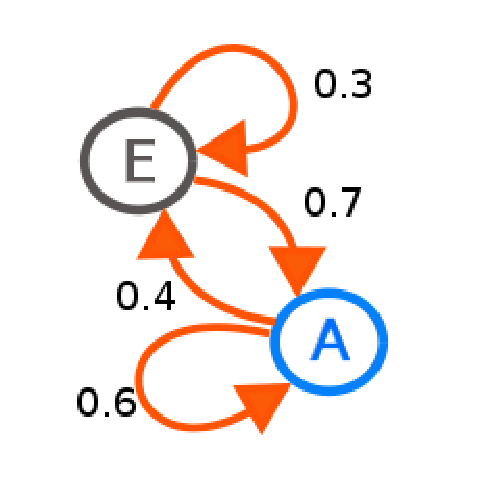
\includegraphics[width=0.6\textwidth]{mcmc1}
    \caption{马尔科夫链}\label{fig:mcmc1}
    \vspace{\baselineskip}
    \end{figure}

  马尔科夫链是描述一类重要的随机动态系统(过程)的模型,系统在每个时期所处的状态是随机的,下一个时间的状态从当前时间状态的
转移是按照一个的概率发生转移的,下个时间点的状态只与本时期的状态和转移概率有关,本质上讲马尔科夫链是时间,状态均为离散的随
机转移过程。

马尔科夫链是随机变量$X_1$,$X_2$,$X_3$,\ldots,的一个数列。这些变量的范围,即他们所有取值的集合,被称为
"状态空间",而$X_n$的值则是在时间n的状态。如果$X_{n+1}$对于过去状态的条件概率分别仅是$X_n$的一个函数,则可以得到
马尔科夫性质,其中X为某个时刻的某种状态: $$P(X_{n+1} = X|X_0,X_1,X_2,\ldots,X_n)=P(X_{n+1} = X|X_n) $$
    
    综合而说,马尔科夫链具有以下特点:可还原性,其本身可以由一个条件分布来表示
$ P(X_{n+1}|X_{n})$,可看作为随机过程中的"转移概率",更多的转移概率可以从一步转移概率,例如
\[ P(X_{n+2}|X_n) =  \int P(X_{n+2},X_{n+1}|X_n) \,dX_{n+1} = \int P(X_{n+2}|X_{n+1}) P(X_{n+1}|X_n) \,dX_{n+1}\]  
马尔科夫链同时具有周期性,重现性,各态遍历性,律动性.

    马尔科夫链的转移概率矩阵说明了马尔科夫的概率,假设$X_n=a_i$的状态概率可表示为 $P_i(n)=P(X_n=a_i)$马尔科夫链的
统计特性不仅仅包含了状态概率,还包含了状态转移概率.$t_s$在$a_i$条件下
,在时间节点$t_n$到达$a_j$状态的条件概率可表示为状态转移概率,记为$P_{ij}(s,n)$
    \[ P_{ij}(s,n)=P{\frac{X_n=a_j}{X_s=a_i}} \]  
    由转移概率可构成转移矩阵
    \[ P(s,n) = \left | \begin{array}{cccc}
        P_{11}(s,n) & P_{12}(s,n)  & \ldots &P_{1N}(s,n) \\
        P_{21}(s,n) & P_{22}(s,n)  & \ldots &P_{2N}(s,n) \\
        \ldots      & \ldots      & \ldots & \ldots    \\
        P_{N1}(s,n) & P_{N2}(s,n)  & \ldots &P_{NN}(s,n) \\
        \end{array} \right| \]

    马尔科夫链的一个性质是收敛的行为与初始概率无关,只与概率转移矩阵有关,当链足够长时,最终到达的收敛终点都是一样的.
这是所有马尔科夫链共有的性质.如下为马尔科夫链的收敛定理:
    
    如果一个非周期马尔科夫链具有转移概率矩阵$P$,且它的任何两个状态是连通的,那么$\lim_{x \rightarrow \infty} P_{ij}^{n}$的存在且与
$i$无关,记$lim_{x \rightarrow \infty}P_{ij}^{n}=\pi(j)$,有

    \begin{displaymath}
        lim_{x\to\infty} = \left[
\begin{array}{ccccc}
\pi(1) & \pi(2) & \ldots & \pi(j) & \ldots \\
\pi(1) & \pi(2) &  \ldots & \pi(j) & \ldots \\
 \ldots& \ldots& \ldots& \ldots& \ldots \\
\pi(1) & \pi(2) &  \ldots & \pi(j) & \ldots \\
 \ldots& \ldots& \ldots& \ldots& \ldots \\
\end{array} \right]
    \end{displaymath}

    其中
    \begin{enumerate}
    \item $\pi(j)=\sum_{i=0}^{\infty}\pi(i) P_{ij}$
    \item 其中$\pi$是马尔科夫链的平稳分布,$$\pi = [\pi(1),\pi(2),\ldots,\pi(j),\ldots],\sum_{i=0}^{\infty}\pi_i=1$$
    \end{enumerate}
    \vspace{1ex}

    关于马尔科夫链的应用,举例说明,某个城市2009年居民的出行方式所占比例做了调查,结果如下bus 21\%,bicycle21\%,
walk 50\% ,car 8\%,这是一个时间齐次的马尔科夫链,

    \begin{table}[htbp]
    \centering  % 表居中
    \begin{tabular}{lcccc}  % {lccc} 表示各列元素对齐方式,left-l,right-r,center-c
    \hline
    &bus&bicycle&walk&car\\ \hline  % \hline 在此行下面画一横线
    bus&90&4&2&4\\
    bicyle&7&86&1&6\\
    walk&8&7&80&5\\
    car&10&2&3&85\\ \hline
    \end{tabular}
    \caption{出行转换比例}
    \end{table}
    
    得出2013年的出行人数总数,可以根据算法步骤,
    \begin{enumerate}
    \item 标识转移矩阵
    \item 初始化概率矩阵
    \item 得出下一年的概率,为当年分配概率和转移矩阵的乘积
    \item 总人数乘以概率可得
    \end{enumerate}

    马尔科夫链在众多科学中都有应用,如统计中可用来建模排队理论和统计学中的建模,也可以做为
算数编码,马尔科夫链也可以用于生物学,用来做基因预测比对排序等功能,同时在网页排序算法中
也可以得到应用,预测用户的互联网浏览行为,作出合理的机器判断.总结来说,马尔科夫过程是
发展迅速,应用广泛的重要随机过程,在信息处理,通信,自动控制,物理,生物以及各种科学应用中
都有着各种的重要应用。

\section{马尔科夫链蒙特卡洛算法介绍}

    马尔科夫链蒙特卡洛算法(MCMC)是一组算法,使用马尔科夫链从随机分布中取样,之前步骤作为底本。总体来说,步数越多,结果越好。
MCMC方法本质上是使用马尔科夫链的蒙特卡罗积分,其基本思想是:构造一条马尔科夫链使其平稳分布为待估参数的后验分布
,借助产生的后验分布样本,基于马尔科夫链达到平稳分布时的样本(有效样本)运算蒙特卡洛积分运算。

MCMC的基本思想是: 假定有一个分布$p(x)$ ,称为目标分布。若分布$p(x)$非常复杂以至于不能直接
抽样, 一个间接获取样本的办法是选择合适的转移矩阵,来构造一个非周期且不可约的马尔科夫链,其稳态分布为$p(x)$,可以
自动搜索概率分布较大的区域并集中计算资源计算.非周期不可约马尔科夫链的重要性质是:从任意初始状态,
运行足够长的时间(因为马尔科夫链的下一个方位取决于当前状态和随机变量,将所有空间覆盖需要话费大量时间)最终能够达到唯一的平稳状态
,在平稳状态下采样取得样本的统计性质与直接从目标分布采样得到的样本的统计性质一致。


设17px为某一空间,产生的总样本数为n,链条达到平稳时的样本数为n,mcmc方法的基本思路可以总结为:
    \begin{itemize}
    \item 构造马尔科夫链,使样本空间能够收敛到平稳分布35px;
    \item 产生样本:由17px中的某一点25px出发,使用马尔科夫链进行抽样模拟,产生点序列73px
    \item 使用蒙特卡罗积分:任意函数36px的期望估计为180px 
    \end{itemize}

    本文着重研究常见的Gibbs抽样
\section{算法伪代码}
\begin{verbatim}

\end{verbatim}
%\begin{algorithmic}
%\State $test$
%\end{algorithmic}
\section{实验结果}
